\documentclass{article}
\usepackage{geometry}
\usepackage{parskip}
\usepackage{graphicx}
\usepackage{pythonhighlight}
\graphicspath{ {./images/} }
\newcommand{\code}[1]{\texttt{#1}}

\geometry{
  a4paper,
  margin=1in
}

\title{SC4002}

\author{
  Ng Tze Kean\\
  \texttt{U2121193J} \and
  Ng Woon Yee\\
  \texttt{U1234567J} \and
  Yap Shen Hwei\\
  \texttt{U1234567J} \and
  Lim Boon Hien\\
  \texttt{U1234567J} \and
  Phee Kian Ann\\
  \texttt{U1234567J} \and
  Lim Ke En\\
  \texttt{U2122069L}
}
\date{\today}

\begin{document}

\maketitle

\section*{Introduction}
We will structure this report to discuss the following parts in each section,
and we detail some of the challenges that we faced and how we have overcome
them.

\section*{Part 0}

In part 0
% TODO: part 0

\section*{Part 1}

\subsubsection*{Discussion}

In this part, we prepare the word embeddings for the downstream tasks in the
later part. Before we obtain the word embeddings, we are tasked to process the
training text, mainly to find out the vocabulary size and out-of-vocabulary
(OOV) words.

To start off, we first used a simple regex approach from GPT2 to extract the
tokens from the text. We then compared the tokenization process with the NLTK
tokenizer and found that the NLTK tokenizer is more accurate in tokenizing the
text.

% TODO: Add more details on the tokenization process and comparison

With that in mind, we decided to use the NLTK tokenizer to tokenize the text.
Next, we opted to use GloVe as the word embeddings for this task. A simple
extraction of the vocabulary size of GloVe is easily done though iterating and
extracting the keys of the embeddings.

To obtain the OOV words, we compared the vocabulary of the training data with
the vocabulary of GloVe through a set difference operation. We defined several
functions to load and tokenize the training set which will be used subsequently
in the other parts. To conclude part 1, we inherit the embeddings from GloVe
and first ignore the OOV words as they will be subsequently handled in part 3.

\subsubsection*{Answer to questions}

\begin{enumerate}
    \item Vocabulary Size: The size of the vocabulary is $18030$, after removing the OOV
          words from Glove embeddings, the final size of the vocabulary is $16163$.

    \item Out-of-Vocabulary (OOV) Words: We identified 1867 OOV words in our training
          data. These words were present in the training data but not found in the GloVe
          dictionary

    \item Mitigating OOV Limitations: To mitigate the issue of OOV we first considered
          the use of <UNK> token to represent all OOV words. However, this approach may
          not be ideal as it does not capture the semantics of the OOV words. Instead, we
          decided to to use character-level embeddings to represent OOV words, this is
          seen in FastText where each word is broken down into character n-grams. This
          approach allows us to capture valid words that might not be in the vocabulary.

          We showcase the snippet of the \code{<UNK>} token code below:

\begin{python}
# mapping of words to indices and vice versa
word2idx = {word: idx for idx, word in enumerate(sorted(vocab))}
idx2word = {idx: word for word, idx in word2idx.items()}

print("Building embedding matrix...")
vocab_size = len(word2idx)
print(f"Vocab size: {vocab_size}")
embedding_matrix = np.zeros((vocab_size, EMBEDDING_DIM))

for word, idx in word2idx.items():
    embedding_matrix[idx] = glove_dict[word]

# add random vector for unknown words
embedding_matrix[word2idx[UNK_TOKEN]] =\
    np.random.normal(scale=0.6, size=(EMBEDDING_DIM,))
\end{python}

\end{enumerate}

\section*{Part 2}

\subsubsection*{Discussion}

\subsubsection*{Answer to questions}

\section*{Part 3}

\subsubsection*{Discussion for 1}

As stated by the task, we unfreeze the word embeddings of the RNN model,
allowing for updates as the model trains. This is done by passing a parameter
to the RNN model to set \code{freeze} to \code{False}. We then train the model
with the train data and evaluate the model with the test data to obtain the
accuracy and loss of the model.

\subsubsection*{Answer to question 1}

% attach image of accuracy and loss graph

\subsubsection*{Discussion for 2}

We apply the mitigation of OOV words by first using the \code{<UNK>} token to
represent all OOV words. Tokens from the train data that are in the GloVe
dictionary will have its embedding taken, and those that are not will be
removed from the vocabulary allowing it to be implicitly represented by the
\code{<UNK>} token. The \code{<UNK>} token will then be assigned a random
embedding vector of the same dimension as the GloVe embeddings.

We also have to modify the model to handle OOV words. This is done in the
forward pass of the model where we check if the word is in the vocabulary. If
it is not, we will use the \code{<UNK>} token to represent the word.

Next, we try to implement the FastText model as the embedding layer to replace
the GloVe embeddings. To aid us in the implementation, we use gensim library to
load the FastText model and then we train the model again with the unfreezed
embedding to obtain the accuracy and loss of the model.

\subsubsection*{Answer to question 2}

With the inclusion of the \code{<UNK>} token and modification of the model
in handling OOV words, the accuracy and loss is as shown below.

% attach image of accuracy and loss graph

With the FastText model, the accuracy and loss is as shown below.

% attach image of accuracy and loss graph

\subsubsection*{Discussion for 3.1}

\subsubsection*{Answer to question 3.1}

\subsection*{Discussion for 3.2 - BiGru Model}
BiGRU model stands for Bidirectional Gated Reccurent Unit, which is a type of
recurrent neural network (RNN). Similarly to LSTM, GRU is designed to model
sequential data by allowing information to be selectively remembered or
forgotten over time. However, in GRU, the memory cell state is replaced with a
"candidate activation vector", which is updated using two gates: the reset gate
and update gate. The reset gate determines how much of the previous hidden
state to forget while the update gate determines how much of the candidate
activation vector to incorporate into the new hidden state.

Therefore, the GRU consists of two gates:
\begin{itemize}
    \item Update gate z that selects whether the hidden state is to be updated with a new
          hidden state.
    \item Reset gate that decides whether previous hidden state is ignored.
\end{itemize}

In this implementation, Spatial dropout is used. The spatial dropout will
zeroes out the entire 1D feature map from the embedding feature vector of each
word, helping in regularisation.

After the GRU layer, we will concatenate both, the average pooling and max
pooling of the hidden representation and the last hidden state of GRU in order
to prevent our model from forgetting informations.
\begin{figure}
    \centering
    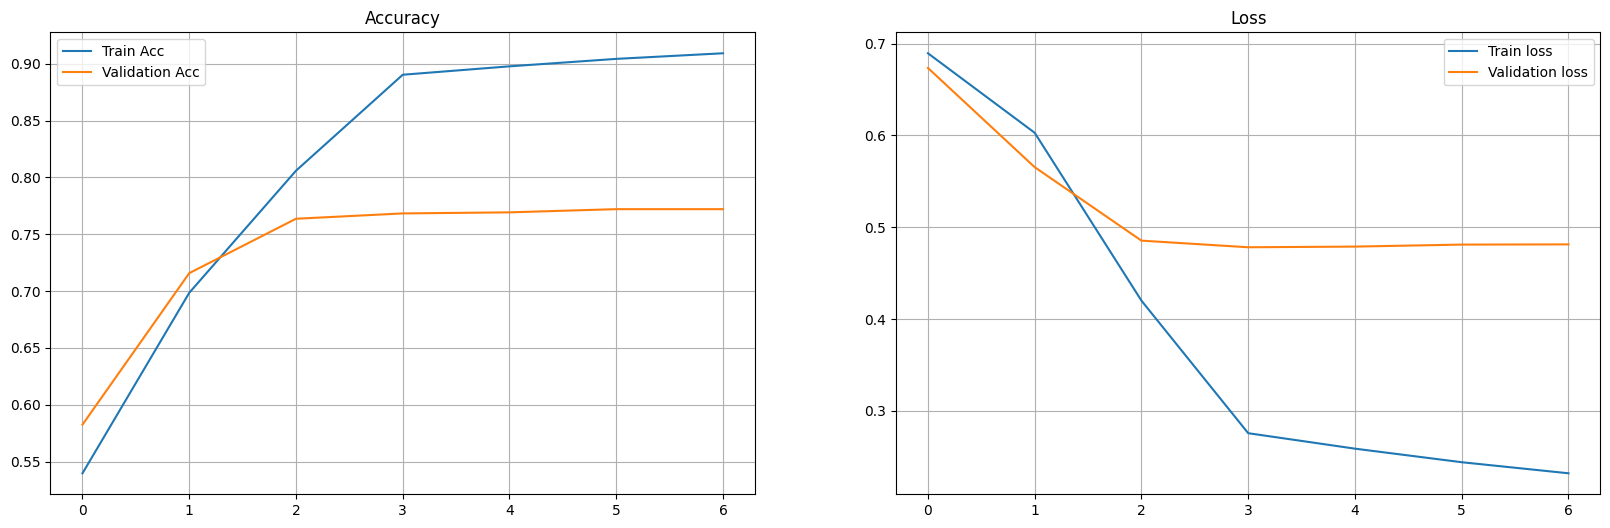
\includegraphics[width=1\linewidth]{BiGRU.png}
    \caption{Accuracy and Loss Data}
    \label{fig:enter-label}
\end{figure}

\subsection*{Answer to question 3.2}
Accuracy scores of BiLSTM and BiGRU model:
\begin{center}
    \begin{tabular}{ | c | c | }
        \hline
        Model  & Test Accuracy     \\
        \hline
        BiLSTM & [bilstm accuracy] \\
        \hline
        BiGRU  & 0.7992            \\
        \hline
    \end{tabular}
\end{center}

Compare the accuracy between BiGRU and BiLSTM

\subsubsection*{Discussion for 4}

\subsubsection*{Answer to question 4}

\section*{Conclusion}
% ...

\end{document}